\documentclass[oneside]{memoir}

\usepackage{graphicx}
\usepackage[usenames,dvipsnames]{xcolor}
\usepackage{booktabs}
\usepackage{listings}

\renewcommand\chaptitlefont{\itshape\Huge\leavevmode\color{BrickRed}}
\renewcommand\printchaptertitle[1]{\raggedleft\chaptitlefont #1 \rule{5mm}{0mm}}
\setsecheadstyle{\hspace{-12mm}\Large\bfseries\color{MidnightBlue}}
\setsubsecheadstyle{\hspace{-12mm}\color{MidnightBlue}}
\setsubsubsecheadstyle{\color{MidnightBlue}}

\setcounter{secnumdepth}{-1}

\begin{document}

\lstset{language=Python}
 
% title page
 
% revision history

\frontmatter
\setcounter{secnumdepth}{-1}

{\raggedleft
%\rule{20mm}{20mm}\\
\hfill Swabian Instruments
}\\
TimeTagger\\
Ultra fast pico second time-to-digital conversion.
\pagebreak\\
Software documentation, examples and related materials are\\[1em]
Copyright 2008-2014 Helmut Fedder\\[1em]
All rights reserved. Unauthorized duplication, in whole or part, of this document by any means except for brief
excerpts in published reviews is prohibited without the express written permission of Helmut Fedder.
Linux is a registered trademark of Linus Torvalds. Microsoft and Windows are both registered trademarks of
Microsoft Corporation. All other trademarks referenced herein are the property of their respective owners and no
trademark rights to the same are claimed.\\[1em]
Revision History:\\
\begin{tabular}{ll}
2013-05-24 & initial release\\
2014-08-27 & corrected variable names\\
\end{tabular}
\pagebreak


\mainmatter
\setcounter{secnumdepth}{-1}

\tableofcontents

\chapter{Introduction}

\begin{center}
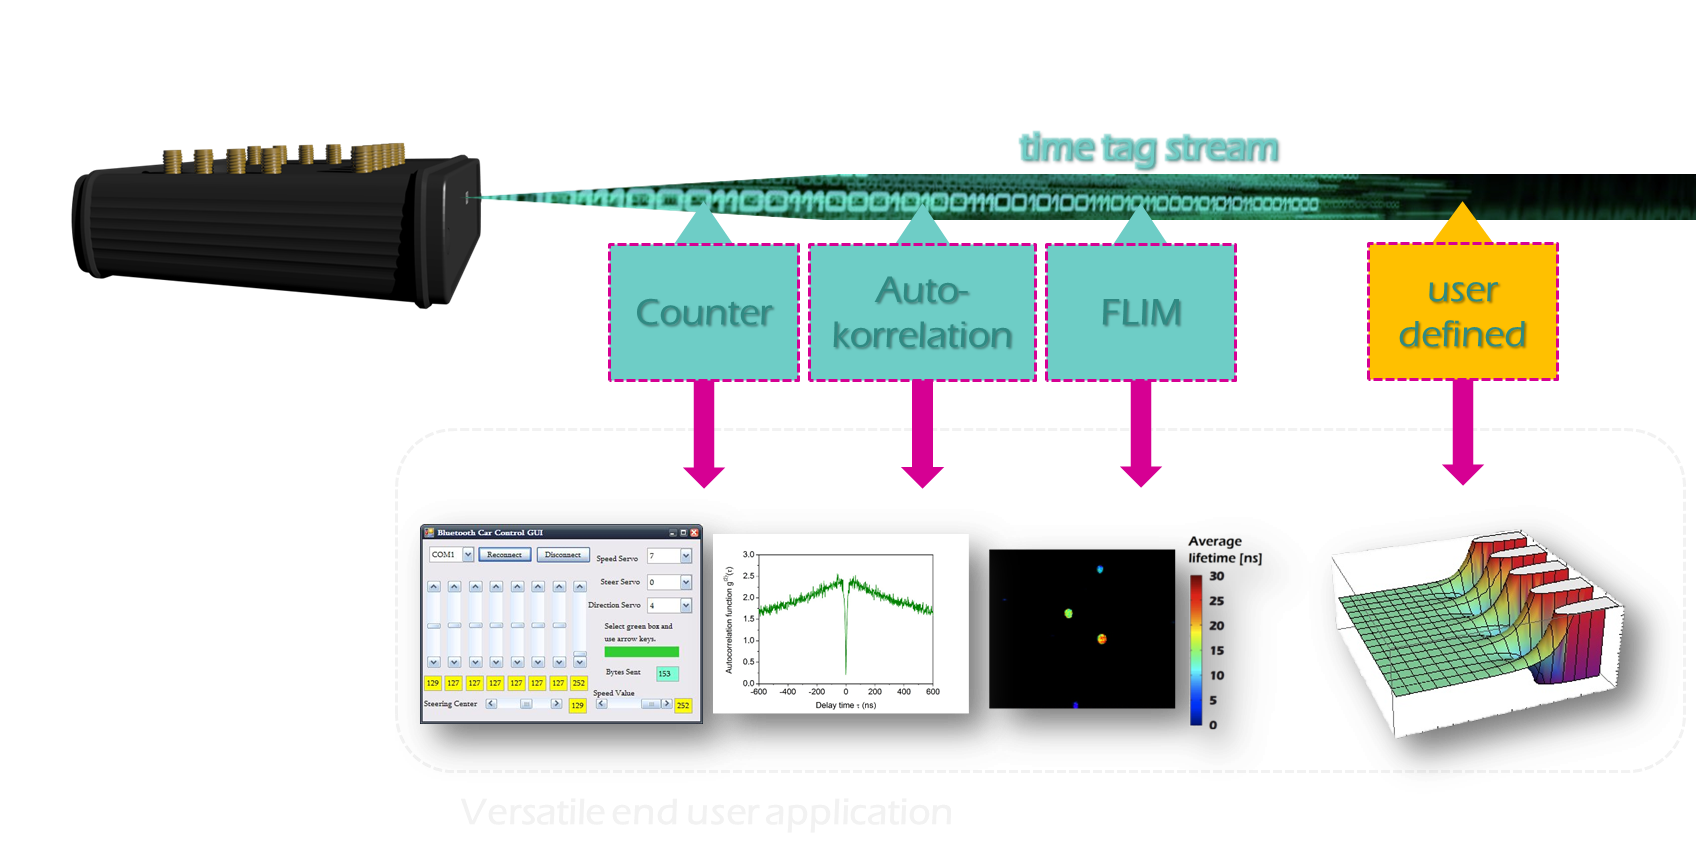
\includegraphics[scale=0.4]{figures/architecture.png}
\end{center}

% figure illustrating the SCPI / web daemon

TimeTagger is a versatile fully USB powered 8-channel time-to-digital converter
with $<$60 ps resolution. It converts rising and falling edges on
the input channels into time tags that are continuously streamed
to a computer via USB. A software backend receives the tags and
analyzes the data stream. Measurement threads hook onto
the time tag stream in a parallel fashion
and analyze the data on-the-fly. The figure above illustrates the architecture.
A set of common measurements is readily provided by the backend, including
counters, time traces, auto-correlation, cross-correlation and fluorescence lifetime
imaging (FLIM). The backend interfaces with various programming
languages, including c++, Python, Java, Matlab and Labview. In addition, the
user can implement custom measurements via a c++ API.

\chapter{Hardware}

\subsection{Data connection}

A USB connection is used for data and power supply. Please ensure that the USB port is capable of providing the full
specified current (500 mA). A USB 2.0 data connection is required for reasonable performance. Operating the device via
a USB hub is strongly discouraged.

\subsection{Input channels}

The TimeTagger has 8 SMA connectorized input channels numbered 0 to 7 throughout this document. The electrical
characteristics are tabulated below. Both rising and falling edges are detected on the input channels.
On the software level, rising edges correspond to channel numbers 0 to 7 and falling edges correspond to
respective channel numbers 8 to 15. Thereby, you can treat rising and falling edges in a fully equivalent fashion.
\subsubsection{electrical characteristics}
\begin{tabular}{ll}
  Termination & 50 $\Omega$\\
  Input voltage range & 0 to 5 V\\
  Trigger level range & 0 to 3.3 V\\
  Minimum signal level & $\sim$30 mV\\
  Minimum pulse width & $\sim$1 ns\\
\end{tabular}

\subsection{Laser synchronization filter}

In a typical fluorescence lifetime application, a target is stimulated with laser pulses with
a fast repetition rate, typically in the 10 to 100 MHz range. Electrical synchronization pulses
are generated that are simultaneous with the excitation laser pulses and are sent to
the TimeTagger along with the single photon signals detected from the target. Because the
data rate of the synchronization pulses is so high, streaming and processing all generated
time tags by the computer is not feasible - and not necessary, since only those synchronization
pulses are of interest that are followed by a photon event. It is therefore desirable
to discard all synchronization time tags in the data stream except those that are followed by a photon.
Since the synchronization pulses are periodic with a very well defined period, it is equivalent
to keep only those synchronization time tags that follow a photon.

This feature is implemented by the onboard event filter that is currently hardcoded between
channel 0 and channel 7. It is assumed that photon clicks are entering channel 0 and laser sync clicks
are entering channel 7. When the filter is active, time tags on channel 7 are only passed
if a time tag has been registered on channel 0 before. Subsequent tags are discarded until the next
tag on channel 0 is detected.

\subsection{General purpose IO (available upon request)}

The device is ready to be equipped with up to four SMA connectorized general purpose IO ports. These can be used
to implement custom features such as special fast input or output triggers, enable / disable gates,
software controllable input and output lines, etc.. Please contact us for custom designs.

\chapter{Software}

The heart of the TimeTagger software is a multi-threaded driver
that receives the time tag stream and feeds it to all running
measurements. Measurements are small threads that analyze the time tag stream
each in their own way. E.g., a count rate measurement will extract all time
tags of a specific channel and calculate the average number of tags received per
second, a cross-correlation measurement will compute the cross-correlation between two
channels, typically by sorting the time tags in histograms, etc.. This is a
powerful architecture that allows you to perform any thinkable time domain
measurement in real time.

\subsection{Web application and JSON-RPC interface}
The easiest way of using the TimeTagger is via a web application
that allows you to interact with the hardware interactively and create
measurement threads and plot the resulting data in a web browser.
You can create an unlimited number of measuremnts
in parallel, plot interactively, save and load data, dump the time tag
stream to a file, etc.. Refer to the subsequent chapter ``quick start'' and
to chapter\ref{sec:WebApplication} if you plan to use the TimeTagger in this
way.

\subsection{precompiled libraries and high level language bindings}
We have implemented a set of typical measurements including count rates, auto
correlation, cross correlation, fluorescence lifetime imaging (FLIM), etc..
For most users, these measurements
will cover all needs. These measurements are included in
the c++ API and provided as precompiled library files. To make using the
TimeTagger even easier, we have equipped these libraries with
bindings to higher level languages including Python, Java, Matlab and Labview
so that you can directly ust the TimeTagger from either of these languages.
With these APIs you can easily start a complex
measurement from a higher level language with only two lines of code. 
To use one of these APIs, you have to write code in the high
level language of your choice. Refer to chapter\ref{sec:API} and the chapter
sepcific to your language if you plan to use the TimeTagger
in this way. 

\subsection{C++ API}
The underlying software architecture is provided by a c++ API that implements
two classes: one class that represent the TimeTagger and one class that
represents a base measurement thread. Ontop of that, the c++ API also provides
all predefined measurement threads that are made available by the web
application and high level language bindings. To use this API, you have to
write and compile a c++ program. If you want to implement a custom
measurement thread you need to follow this approach. Refer to
chapter\ref{sec:API} if you plan to use the TimeTagger in this way.


\chapter{Quick Start}

... for the impatient!

\subsection{Start the web application}

\begin{enumerate}
 \item connect the TimeTagger to a USB port
 \item wait until 'new USB device is ready to use' is displayed in the notification area
 \item run the web server from the start menu Programs $>$ TimeTagger $>$ web server
 \item start a web browser and enter 'localhost:8080' in the navigation bar
\end{enumerate}
A website should be displayed as shown below.
\begin{center}
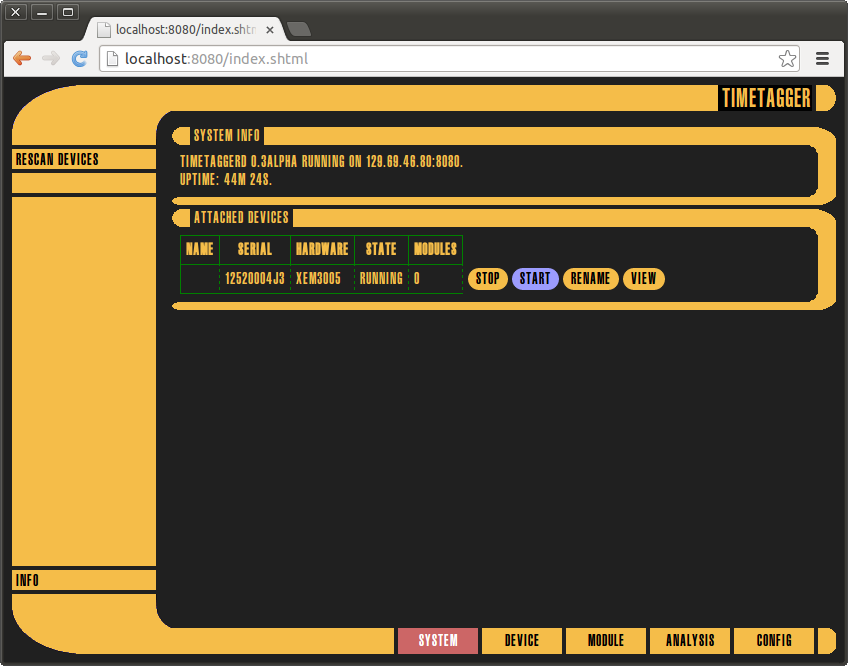
\includegraphics[scale=0.4]{figures/web_application.png}
\end{center}

\subsection{Starting a measurement: a count rate}

\begin{enumerate}
 \item click 'DEVICE' on the bottom
 \item click 'NEW COUNTRATE' on the left
 \item click 'SAVE' in the lower half
 \item click 'VIEW' in the upper half
\end{enumerate}
A bar plot should be displayed that shows the count rates on all channels. By default the trigger levels are set to
0.5 V on all channels. If you have a signal connected to your TimeTagger that exceeds this level, you
should already see the count rate of your signal. Make sure that your signals do not exceed the total data rate of
about 4 M tags / second. If your data rate is too high the value 'overflows' in the 'DEVICE' tab will be larger than
zero. If you have not applied a signal yet, this is a good moment to do so. We will proceed adjusting the trigger
levels.
\begin{center}
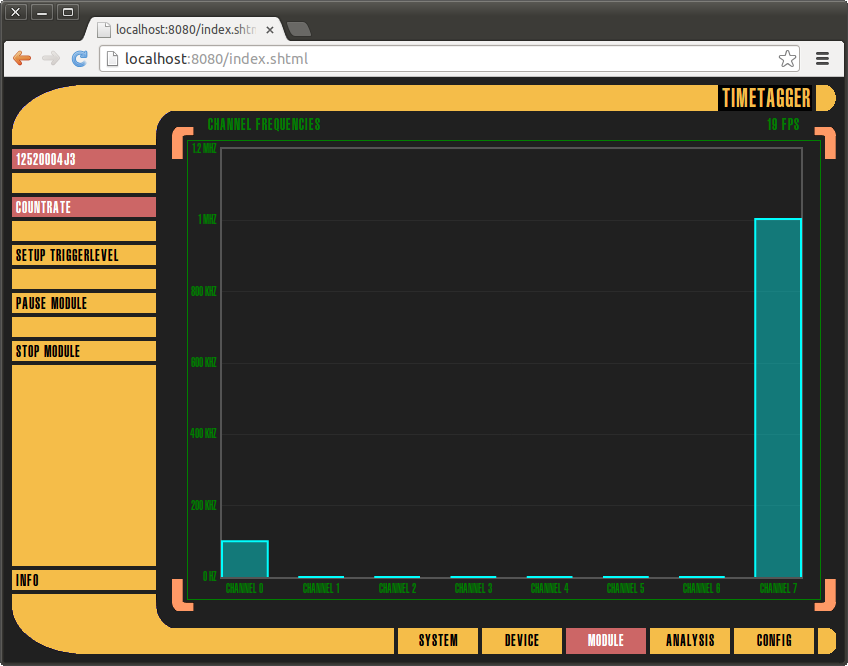
\includegraphics[scale=0.4]{figures/countrate.png}
\end{center}

\subsection{Adjusting the trigger levels}

\begin{enumerate}
 \item click 'SETUP TRIGGERLEVEL' on the left
 \item use the sliders to adjust the triggerlevels to your needs
 %\item you can also enable and disable the laser synchronization filter here,
 %e.g., if you are planning to do a fluorescence lifetime measurement. This
 %feature is a bit subtle. When the filter is active, a time tag on channel 7 is
 %accepted only when there has been a tag on channel 0 beforehand.
 \item click 'CLOSE' when you are done
\end{enumerate}

\subsection{Adding another measurement: a cross-correlation}

\begin{enumerate}
 \item click 'DEVICE' on the bottom
 \item click 'NEW CORRELATION' on the left
 \item specify the channels for your correlation measurement. The thread measures the time differences between a
click on the 'start channel' and all subsequent clicks on the 'click channel' and accumulates them in a histogram
 \item leave the 'sequence channel' set to 'None'
 \item enter the bin width (in ps) and the number of bins to define the histogram resolution and range
 \item click 'SAVE' and 'VIEW'
\end{enumerate}
A line plot should be displayed that shows the cross-correlation function between the two channels you have chosen. The
plot could look similar to the one shown below, that shows an example of a cross correlation between channel 0 and 7
with the default settings and with square waves applied to channels 0 and 7, with frequencies of 100 kHz and 2 MHz,
respectively, resulting in typical delta like peaks.
\begin{center}
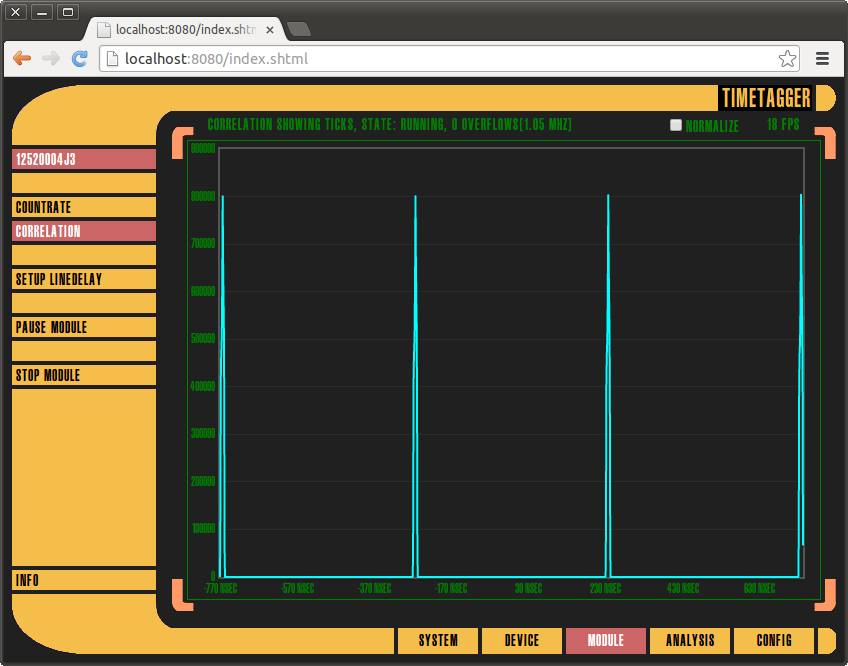
\includegraphics[scale=0.4]{figures/crosscorrelation.png}
\end{center}

\subsection{Save your data}

\begin{enumerate}
 \item click 'STOP MODULE' on the left
 \item click 'SAVE DATASET' on the left
 \item enter a name and additional information according to your needs and click 'SAVE'
\end{enumerate}
The data is saved in .json format, that can be easily interpreted by many 3rd party software
tools (see http://www.json.org/).

% \chapter{Using the TimeTagger}
% 
% The TimeTagger can be accessed via three different interfaces.
% 
% \subsection{Web application}
% A web application provides acquisition and life plotting of typical measurements.
% The web interface is designed to provide an oscilloscope-like experience and navigation.
% 
% \subsection{Python module}
% Typical measurements are also made available via a precompiled python module.
% 
% \subsection{C++}
% The full feature set, in particular the possibility to implement custom measurements,
% is provided by a C++ API.
% 
% \subsection*{}
% In the following, we first discuss the underlying API. The higher level interfaces are discussed further down.
% 
% 

\chapter{Application Programmer's Interface}\label{sec:API}

The API provides methods to control the hardware and to create
measurements that are hooked onto the time tag stream. It is written in C++ but
wrapper classes are provided in higher level languages including python and
Java, that can directly be used in your application, in a way that is equivalent
to the C++ classes. The API includes a set of typical measurements that will
cover most needs. Implementation of custom measurement threads is based on
subclassing from a C++ base class and thus is only available in the C++ API.

\subsection{API documentation}

The API documentation in this manual gives a general overview how to use the TimeTagger.
More detailed information can be found in the API reference (generated with
Doxygen).
% ToDo path do reference

\subsection{Samples}

Often the fastest way to learn how to use an API is by means of examples. Please see the 'samples'
subfolder of your TimeTagger installation for examples.

\subsection{Units}

Time is measured in ps since device startup and represented by 64 bit integers. Note that this
implies that the time variable will overflow once after about 0.83 years. This
will most likely not be relevant to you unless you plan to run your software
continuously over one year and are taking data at the instance when the overflow is happening.

\subsection{Rising and falling edges}

You can use the TimeTagger to detect both rising and falling edges. Throughout
the software API, the rising edges are represented by channels 0 to 7 and
the falling edges are represented by channel numbers 8 to 15.

\section{Organization}

The API contains a small number of classes which you instantiate in your code.
These classes are summarized below.
\subsubsection{Classes}
\begin{tabular}{p{0.28\textwidth}p{0.6\textwidth}}
  TimeTagger & Represents the hardware and provides methods to control the trigger levels and data filter.\\
  Iterator & Base class for implementing custom measurements.\\
  Countrate & Average click rate on one or more channels.\\
  Counter & Counts clicks on one or more channels with a fixed binwidth and
  circular buffer output.\\
  CountBetweenMarkers & Counts click on one channel where the bins are
  determined by triggers on one or two other channels. Uses static buffer
  output. Use this to implement a gated counter, a counter synchronized to
  an external sampling clock, etc.\\
  TimeDifferences & Accumulates the time differences between clicks on two
  channels in one or more histograms. The sweeping through
  histograms is optionally controlled by one or two additional triggers.\\
  Histogram & A simple histogram of time differences. This can be used e.g.
  to measure lifetime.\\
  Correlation & auto- and cross-correlation.\\
  FLIM & Fluorescence lifetime imaging.\\
  StartStop & Accumulates a histogram of time difference between
  pairs of clicks on two channels. Only the first stop click after a start click is
  considered. Subsequent stop clicks are discarded. The Histogram length is
  unlimited.\\
\end{tabular}
\subsubsection*{}
The TimeTagger class is provided in a dynamically linked library that is located in the
'windows{\textbackslash}system' folder. Measurement threads are provided as C++ source code in the
'api' subfolder of your TimeTagger installation.

\section{The TimeTagger class}

This class provides access to the hardware and exposes methods to control hardware settings.
Behind the scenes it opens the USB connection, initializes the device
and receives the time tag stream. Every measurement requires an
instance of the TimeTagger class to which it will be associated. In a typical application
you will perform the following steps:
\begin{enumerate}
 \item create an instance of TimeTagger
 \item use methods on the instance of TimeTagger to adjust the trigger levels
 \item create an instance of a measurement passing the instance of TimeTagger to the constructor
\end{enumerate}
You can use multiple TimeTaggers on one computer simultaneously. In this case, you usually want to
associate your instance of the TimeTagger class to a physical TimeTagger. To
implement this in a bullet proof way, TimeTagger instances must be created
by a factory function called 'createTimeTagger'. The factory function accepts
the serial number of a physical TimeTagger as a string argument (every
TimeTagger has a unique hardware serial number). The serial number is the only argument that can
be passed. If an mpty string or no argument is passed, the first detected
TimeTagger will be used. To find out the hardware serial number, you can connect
a single timetagger, open it and use the 'getSerial' function described below.

The TimeTagger class contains a small number of methods to control the hardware settings that are summarized below.
\subsubsection{Methods}
\begin{tabular}{p{0.25\textwidth}p{0.6\textwidth}}
  setTriggerLevel & set the trigger level of an input channel\\
  getTriggerLevel & return the trigger level of an input channel\\
  setLineDelay & set the input delay of a channel\\
  getLineDelay & return the input delay of a channel\\
  setFilter & enable or disable the laser synchronization filter (currently hardcoded between channel 0 and 7)\\
  getFilter & return the state of the laser synchronization filter\\
  setNormalization & activate or deactivate gaussian normalization of the
  detection jitter\\
  getNormalization & return whether input normalization is turned on\\
  setNormalization & return whether input normalization is turned on\\
  getDeadTime & return the dead time of a channel\\
  setDeadTime & set the dead time of a channel\\
  enableCalibration & apply internal test signal to a channel\\
  disableCalibration & deactivate internal test signal on a channel\\
  getSerial & return the hardware serial number\\
\end{tabular}

\section{Analysis threads}

The TimeTagger derives its versatility from the flexible analysis threads that can be hooked
onto the time tag stream. Any number of analysis threads can be instantiated and run in parallel in a
multithreaded fashion. Analysis threads are derived from an 'Iterator' base class described
further down that can be used to implement new custom analysis threads. A set of
typical measurements has been implemented as part of the library and is also
provided as C++ source code. These analysis threads are briefly described here.

All predefined analysis threads provide a small number of methods to start and stop the excecution
and to access the accumulated data. The methods are summarized below.
\subsubsection{Methods}
\begin{tabular}{p{0.25\textwidth}p{0.6\textwidth}}
  getData & Returns the data accumulated by the thread up to now. The returned data can be a scalar or a multi
dimensional array, depending on the measurement.\\
  clear & enable or disable the laser synchronization filter (currently hardcoded between channel 0 and 7)\\
  start & set the trigger level of an input channel\\
  stop & return the trigger level of an input channel\\
\end{tabular}
\subsubsection*{}
All predefined Analysis threads start accumulating data immediately after their creation.
In a typical application you will perform the following steps:
\begin{enumerate}
 \item create an instance of an anlysis thread, e.g.~a countrate on channel 0
 \item wait for some time
 \item retrieve the data accumulated by the thread up to now by calling the 'getData' method.
\end{enumerate}
The specific measurement threads are described below.

\subsection{Countrate}

Measures the average countrate on one or more channels. Specifically, it
counts incoming clicks and determines the time between the first click since
instantiation and the latest click. The ratio of the number of clicks and the
time corresponds to the average countrate since the first click.
\subsubsection{Arguments}
\begin{tabular}{p{0.25\textwidth}p{0.6\textwidth}}
  channels & <vector int> channels used for counting clicks\\
\end{tabular}
\subsubsection{Methods}
\begin{tabular}{p{0.25\textwidth}p{0.6\textwidth}}
  getData & returns the average countrate in counts per second.\\
  clear & resets the accumulated clicks to zero and uses the next incoming click as the first click.\\
\end{tabular}

\subsection{Counter}

Streaming counter with specific binwidth and vector output. This class
is suitable to generate a time trace of the countrate. Specifically
the thread repeatedly counts clicks on a single channel over a time interval of
length 'binwidth' and stores the results in an array of size 'bins'.
The array is treated as a circular buffer. A new value is shifted in
after a time given by 'binwidth'.
\subsubsection{Arguments}
\begin{tabular}{p{0.25\textwidth}p{0.6\textwidth}}
  channels & <vector int> channels used for counting clicks\\
  binwidth & <longlong> binwidth in ps\\
  n values & <int> number of values\\
\end{tabular}
\subsubsection{Methods}
\begin{tabular}{p{0.25\textwidth}p{0.6\textwidth}}
  getData & returns an array of size 'bins' containing the current values of the circular buffer
  (counts in each bin).\\
  clear & resets the array to zero and restarts the measurement.\\
\end{tabular}

\subsection{CountBetweenMarkers}

Count between hardware triggers with vector output. You can use this thread to record a line-scan (or
two-dimensional image). Specifically, the thread counts clicks on the 'click channel'. When a click
is detected on the marker channel it stores the current counter value as next entry in the output vector,
resets the counter to zero and starts accumulating counts again. The thread stops when all
entries in the output vector are filled.
\subsubsection{Arguments}
\begin{tabular}{p{0.25\textwidth}p{0.6\textwidth}}
  click channel & channel that increases the count\\
  begin channel & channel that triggers beginning of counting and stepping to the next value\\
  end channel & channel that triggers end of counting\\
  n values & the number of values\\
\end{tabular}
\subsubsection{Methods}
\begin{tabular}{p{0.25\textwidth}p{0.6\textwidth}}
  getData & returns an array of size 'bins' containing the acquired counter values.\\
  clear & resets the array to zero and restarts the measurement.\\
  ready & returns 'true' when the entire array is filled.\\
\end{tabular}

\subsection{TimeDifferences}

Accumulates the time differences between clicks on two channels in one or more histograms.
Useful to perform auto- and cross-correlation measurements and more general
time-difference measurements between two channels.
Specifically, the thread waits for a click on the 'start channel', then measures the
time difference between the start click and all subsequent clicks on the 'click channel'
and stores them in a histogram. The histogram has a number of 'bins'
bins of binwidth 'binwidth'. Clicks that fall outside the histogram range are discarded.
Data accumulation is performed independently for all start clicks. This type of measurement is frequently refered to as
'single start, multiple stop' measurement and corresponds to a full auto- or cross-correlation measurement.

The data obtained from subsequent start clicks can be accumulated into the same histogram (one-dimensional measurement)
or into different histograms (two-dimensional measurement). In this way you can perform more general two-dimensional
time-difference measurements. The parameter 'histograms' specifies the number of histograms. After each click
on the start channel, the histogram index is incremented by one (and reset to zero after a number of 'histograms'
start clicks have been received. You can also provide a synchronization trigger that resets the histogram index by
specifying a channel number as argument 'sync channel'.

Typically, you will run the measurement indefinitely until stopped by the user. However, it is also possible to
specify the number of start clicks. In this case the measurement stops itself when the number of start clicks
has reached the specified value. In case of a two-dimensional measurement, it will measure until every histogram
has a seen the specified number of start clicks.

\subsubsection{Arguments}
\begin{tabular}{p{0.25\textwidth}p{0.6\textwidth}}
  click channel & channel that increments the count in a bin\\
  start channel & channel that sets start times relative to which clicks on the click channel are measured\\
  next channel & channel that increments the histogram index\\
  sync channel & channel that resets the histogram index to zero\\
  binwidth & binwidth in ps\\
  n bins & number of bins in each histogram\\
  n histograms & number of histograms\\
\end{tabular}
\subsubsection{Methods}
\begin{tabular}{p{0.25\textwidth}p{0.6\textwidth}}
  getData & returns a two-dimensional array of size 'bins' times 'histograms' containing the histograms.\\
  clear & resets the array to zero.\\
  setMaxCounts & set the maximum number of start clicks accepted\\
  getCounts & returns the number of start clicks\\
  ready & returns 'true' when the required number of start clicks set by 'setMaxCounts' has been reached\\
\end{tabular}

\subsection[*]{Correlation}

Accumulates time differences between clicks on two channels into
a histogram, where all ticks are considered both as start and stop
clicks and both positive and negative time differences are considered.
The histogram is determined by the number of bins and the binwidth, which
are used both for the positive and the negative histogram range (i.e.,
length of the histogram is 2$*$n bins$+$1).

\subsubsection{Arguments}
\begin{tabular}{p{0.25\textwidth}p{0.6\textwidth}}
  channel 1 & first click channel\\
  channel 2 & second click channel\\
  binwidth & binwidth in ps\\
  n bins & the number of bins in the resulting histogram is 2$*$n bins$+$1\\
\end{tabular}
\subsubsection{Methods}
\begin{tabular}{p{0.25\textwidth}p{0.6\textwidth}}
  getData & returns a two-dimensional array of size 'bins' times 'histograms' containing the histograms.\\
  clear & resets the array to zero.\\
  setMaxCounts & set the maximum number of start clicks accepted\\
  getCounts & returns the number of start clicks\\
  ready & returns 'true' when the required number of start clicks set by 'setMaxCounts' has been reached\\
\end{tabular}


\subsection[*]{FLIM}

Fluorescence lifetime imaging. Specifically, the thread performs a single-start-multiple-stop measurement
and accumulates the time differences into a histogram with specified binwidth and number of bins. The condition
for moving to the next pixel can either be a pixel trigger on a third channel or a predefined accumulation
time per pixel. After accumulating a number of 'pixels' histograms, the measurement stops. This measurement
is also useful to record cross-correlation on multiple pixels.

\subsubsection{Arguments}
\begin{tabular}{p{0.25\textwidth}p{0.6\textwidth}}
  click channel & channel that increments the count in a bin\\
  start channel & channel that sets start times relative to which clicks on the click channel are measured\\
  next channel & channel that increments the histogram index\\
  binwidth & binwidth in ps\\
  n bins & number of bins in each histogram\\
  n histograms & number of histograms\\
\end{tabular}

\subsubsection{Methods}
\begin{tabular}{p{0.25\textwidth}p{0.6\textwidth}}
  getData & returns a two-dimensional array of size 'pixels' times 'bins' containing the histograms.\\
  clear & resets the array to zero.\\
  ready & returns 'true' when the measurement is ready\\
\end{tabular}

\subsection[*]{Dump}

Dump the time tag stream to a file in a binary format.

\subsubsection{Arguments}
\begin{tabular}{p{0.25\textwidth}p{0.6\textwidth}}
  filename & name of the file to dump to\\
\end{tabular}

\subsubsection{Methods}
\begin{tabular}{p{0.25\textwidth}p{0.6\textwidth}}
  stop & stop the thread\\
\end{tabular}


\section{Defining custom analysis threads by subclassing Iterator}

The information will be provided shortly.

\chapter{Python module}

The python bindings are one-to-one equivalents of the C++ API. C++ <> vector
arguments translate to python $[]$ lists. 


\chapter{Web application}\label{sec:WebApplication}

\section{Web Daemon / SCPI Interface}

A web daemon is provides that enables easy access to the TimeTagger hardware and
provides acquisition and life plotting of common measurements such as counters,
autocorrelation and fluorescence lifetime imaging (FLIM) via a web browser
and an SCPI interface. The web interface is designed to provide an oscilloscope-like
experience and navigation. Refer to the API section for a detailed explanation
of the provided measurements. The daemon is a stand-alone software piece and ready to use.

% figure illustrating daemon
% screen shot

\end{document}



